在区分因子对比之前,我们先研究了基线算法DL1r的三个输出值$p_b$、$p_c$和$p_u$在样本中的分布,
它们分别代表jet被判定为b-jet、c-jet或者除前两者之外的light-jet的概率,
以及新算法的三个输出值$p_{\text{Higgs}}$、$p_{\text{multijet}}$和$p_{\text{top}}$在样本中的分布,
它们分别代表事例是来自Higgs-jet、QCD-jet和Top-jet事例的概率:
\begin{itemize}
\item 图~\ref{fig:DL1RLD}~分别展示了在信号样本、multijet样本和t夸克样本中,领头LR-jet中的领头VR-jet的DL1r算法输出值$p_b$、$p_c$和$p_u$的分布。
其中左图代表$p_b$的分布,中间的图代表$p_c$的分布,右图代表$p_u$的分布,橙色线代表信号样本,蓝色线代表multijet样本,绿色线代表t夸克样本。
所有分布都已经归一化。
\item 图~\ref{fig:DL1RLLD}~分别展示了在信号样本、multijet样本和t夸克样本中,领头LR-jet中的次领头也就是横动量第二高的VR-jet的DL1r算法输出值$p_b$、$p_c$和$p_u$的分布。
其中左图代表$p_b$的分布,中间的图代表$p_c$的分布,右图代表$p_u$的分布,橙色线代表信号样本,蓝色线代表multijet样本,绿色线代表t夸克样本。
所有分布都已经归一化。
\item 图~\ref{fig:DL1RLLLD}~分别展示了在信号样本、multijet样本和t夸克样本中,领头LR-jet中的次次领头也就是横动量第三高的VR-jet的DL1r算法输出值$p_b$、$p_c$和$p_u$的分布。
其中左图代表$p_b$的分布,中间的图代表$p_c$的分布,右图代表$p_u$的分布,橙色线代表信号样本,蓝色线代表multijet样本,绿色线代表t夸克样本。
所有分布都已经归一化。
\item 图~\ref{fig:DXBBPP}~分别展示了在信号样本、multijet样本和t夸克样本中,领头LR-jet中的新算法输出值$p_{\text{Higgs}}$、$p_{\text{multijet}}$和$p_{\text{top}}$的分布。
其中左图代表$p_{\text{Higgs}}$的分布,中间的图代表$p_{\text{multijet}}$的分布,右图代表$p_{\text{top}}$的分布,橙色线代表信号样本,蓝色线代表multijet样本,绿色线代表t夸克样本。
所有分布都已经归一化。
\end{itemize}
从图中对比可以看到,新算法的输出值在三个样本中的分布差异比较显著。

\begin{figure}[h]
    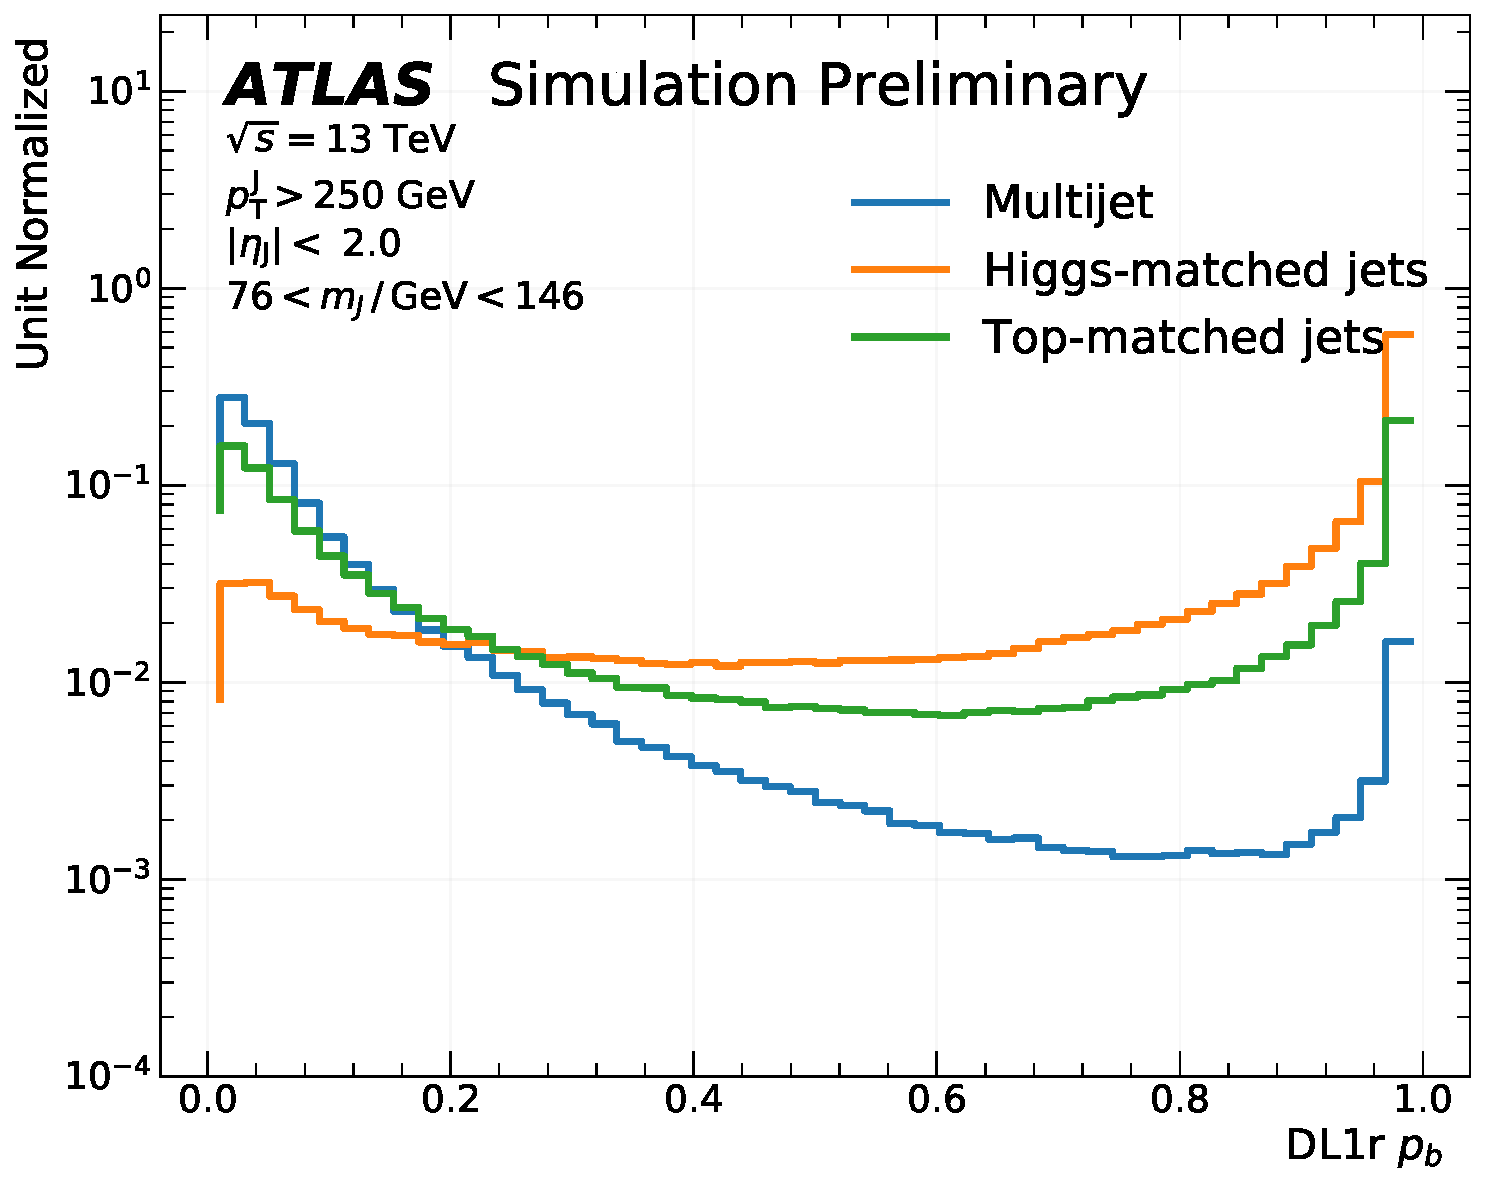
\includegraphics[width=0.33\textwidth]{figuresXbb/samples/inputs_aux/dl1r_pb_1_norm.pdf}
    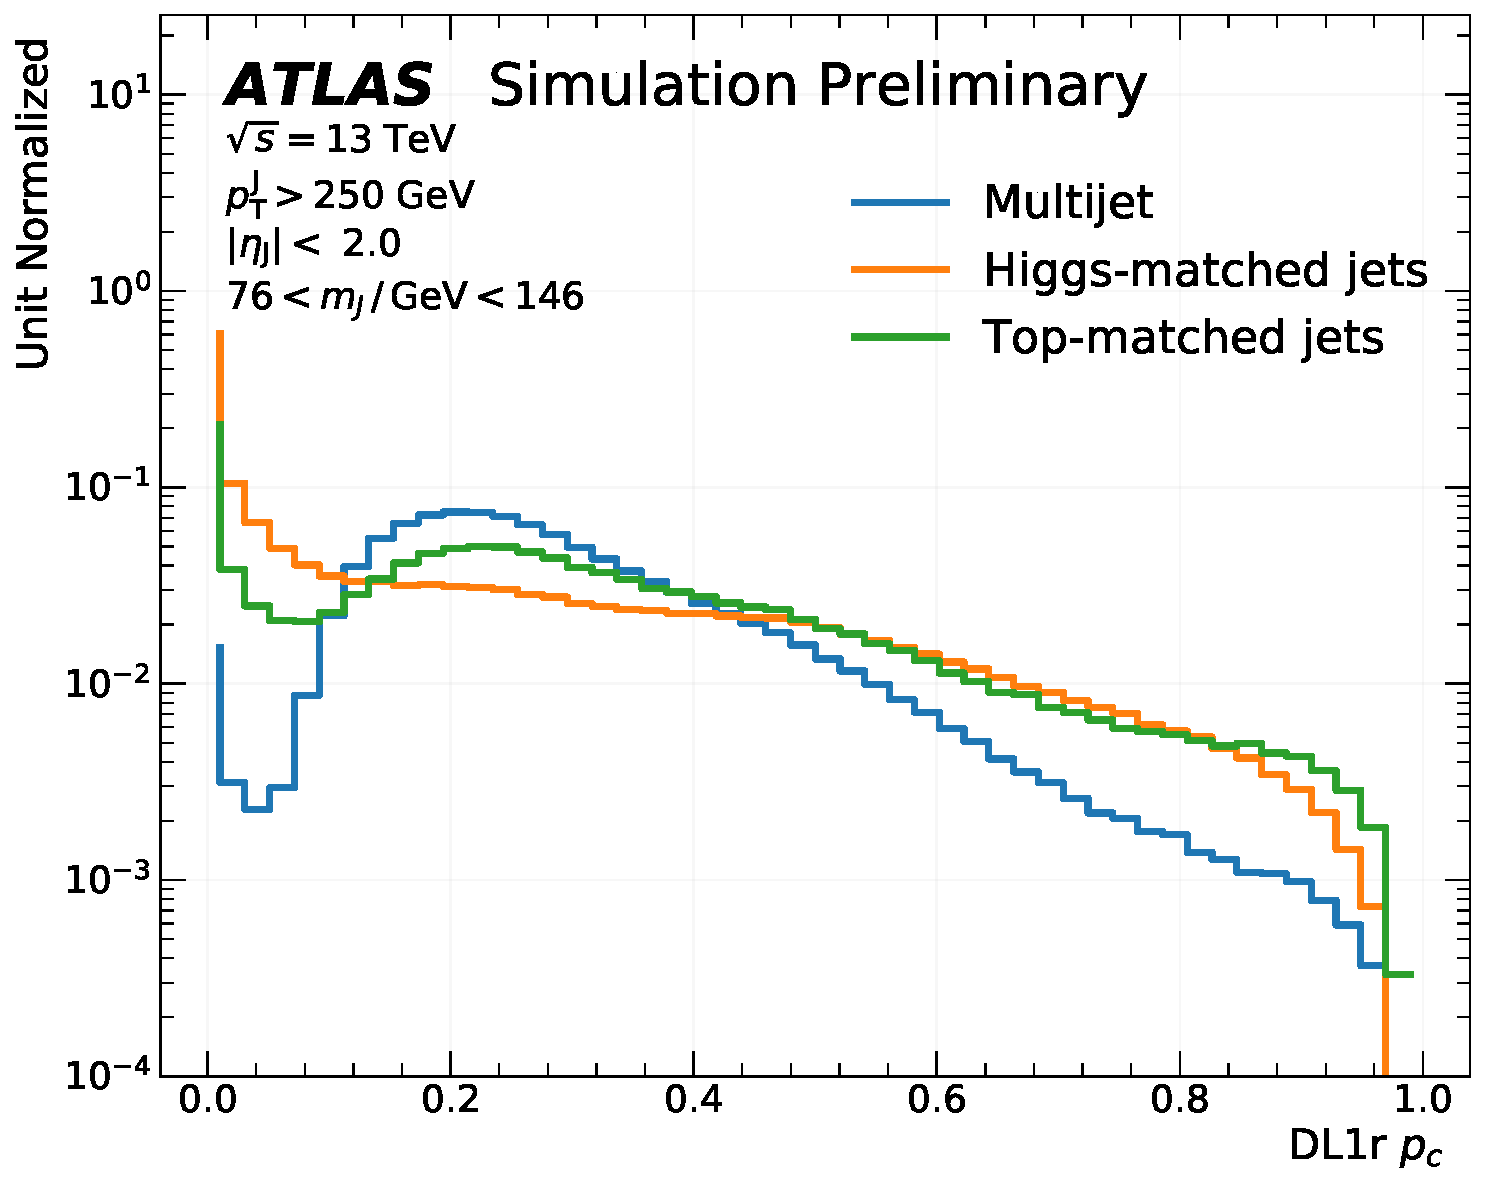
\includegraphics[width=0.33\textwidth]{figuresXbb/samples/inputs_aux/dl1r_pc_1_norm.pdf}
    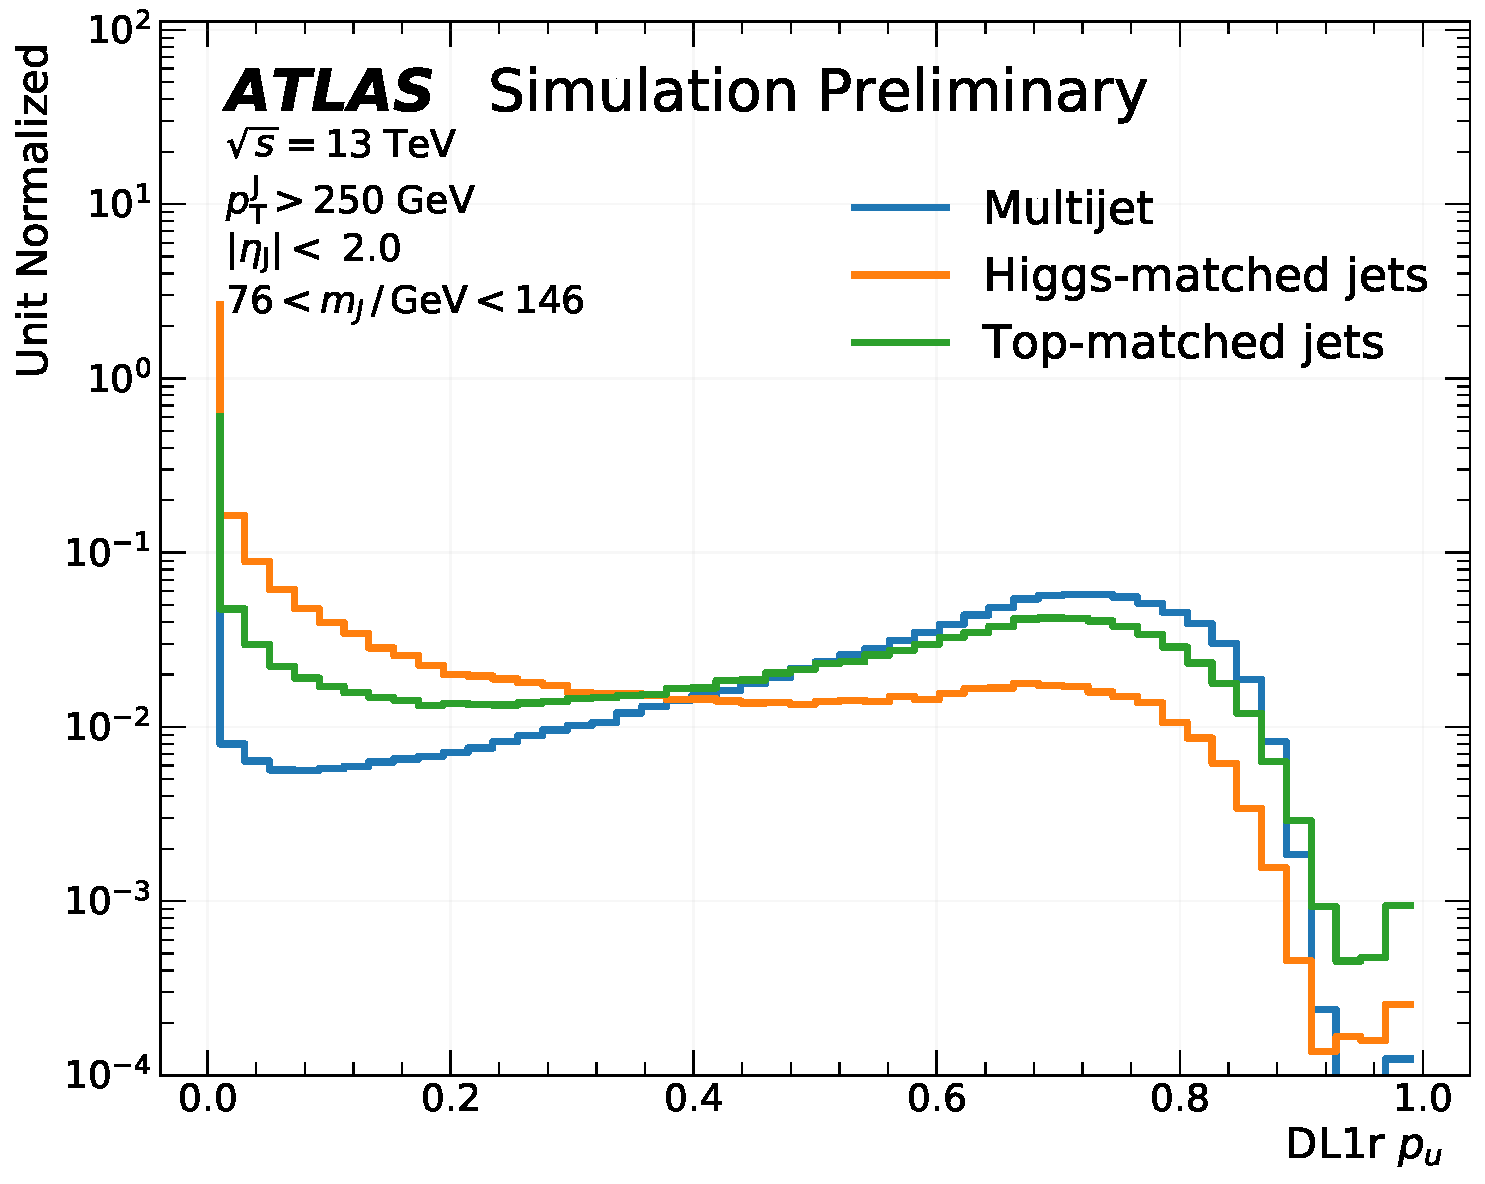
\includegraphics[width=0.33\textwidth]{figuresXbb/samples/inputs_aux/dl1r_pu_1_norm.pdf}
  \caption{在信号样本、multijet样本和t夸克样本中,领头LR-jet中的领头VR-jet的DL1r算法输出值$p_b$、$p_c$和$p_u$的分布。
其中左图代表$p_b$的分布,中间的图代表$p_c$的分布,右图代表$p_u$的分布,橙色线代表信号样本,蓝色线代表multijet样本,绿色线代表t夸克样本。
所有分布都已经归一化。}
  \label{fig:DL1RLD}
\end{figure}

\begin{figure}[h]
    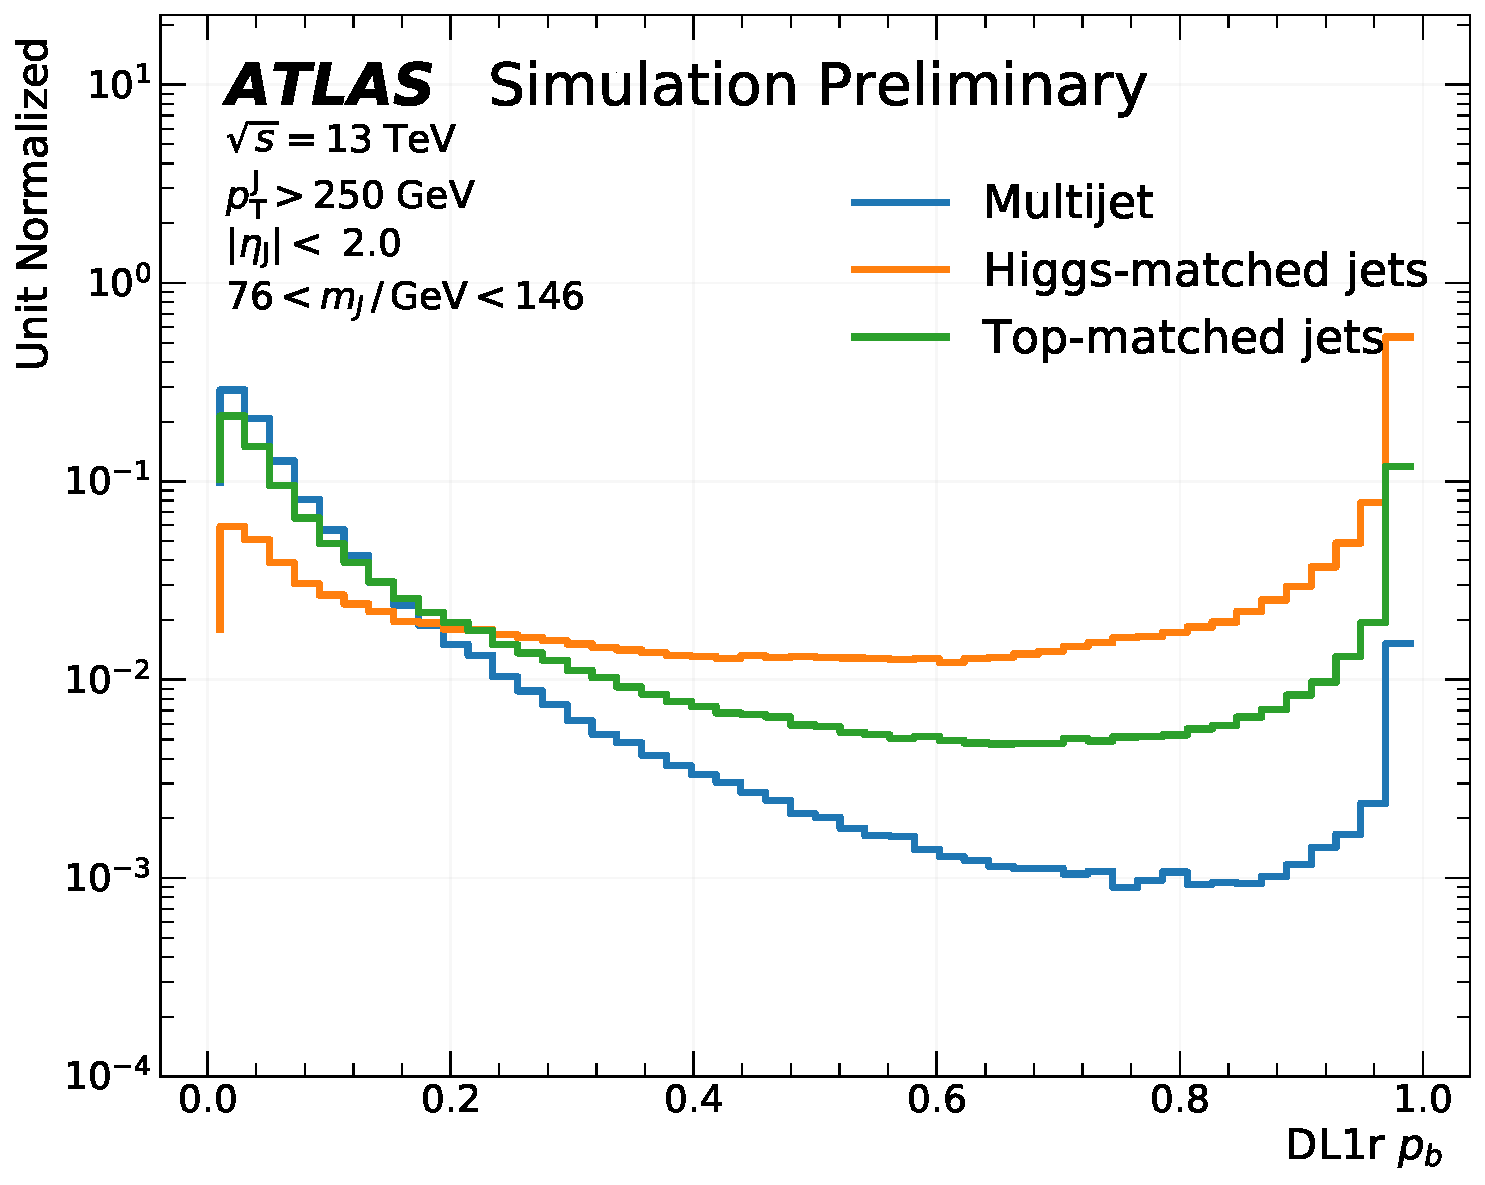
\includegraphics[width=0.33\textwidth]{figuresXbb/samples/inputs_aux/dl1r_pb_2_norm.pdf}
    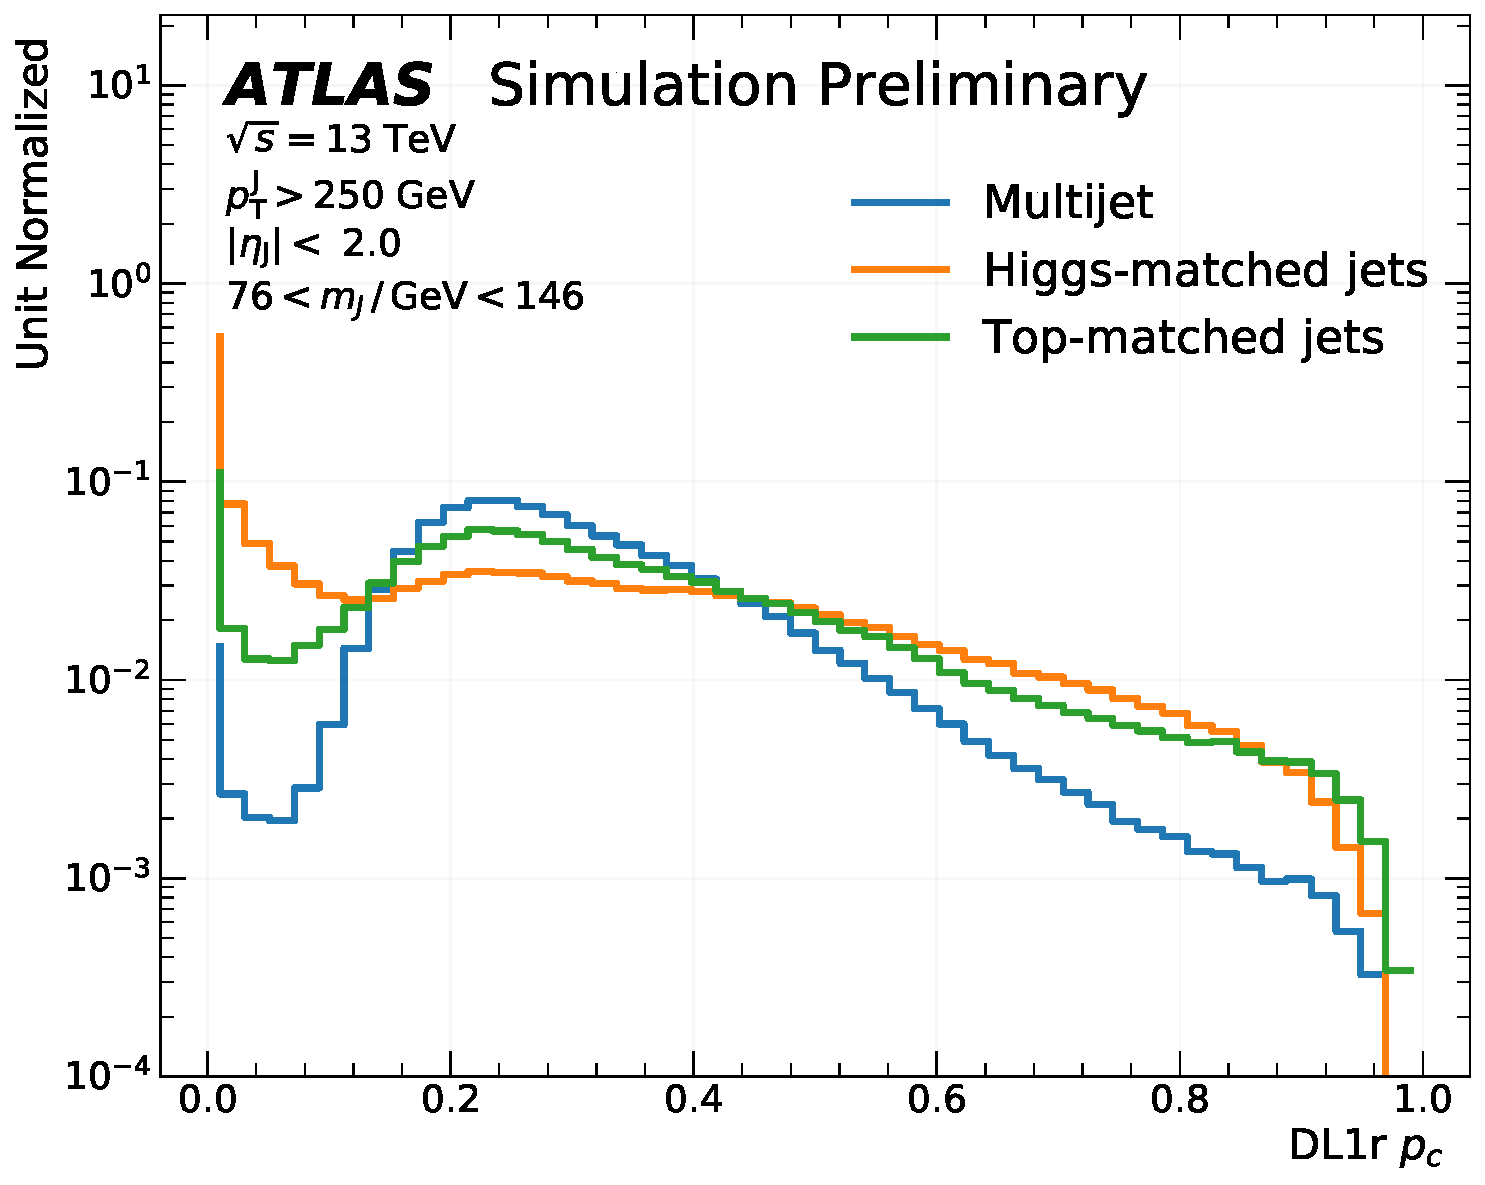
\includegraphics[width=0.33\textwidth]{figuresXbb/samples/inputs_aux/dl1r_pc_2_norm.pdf}
    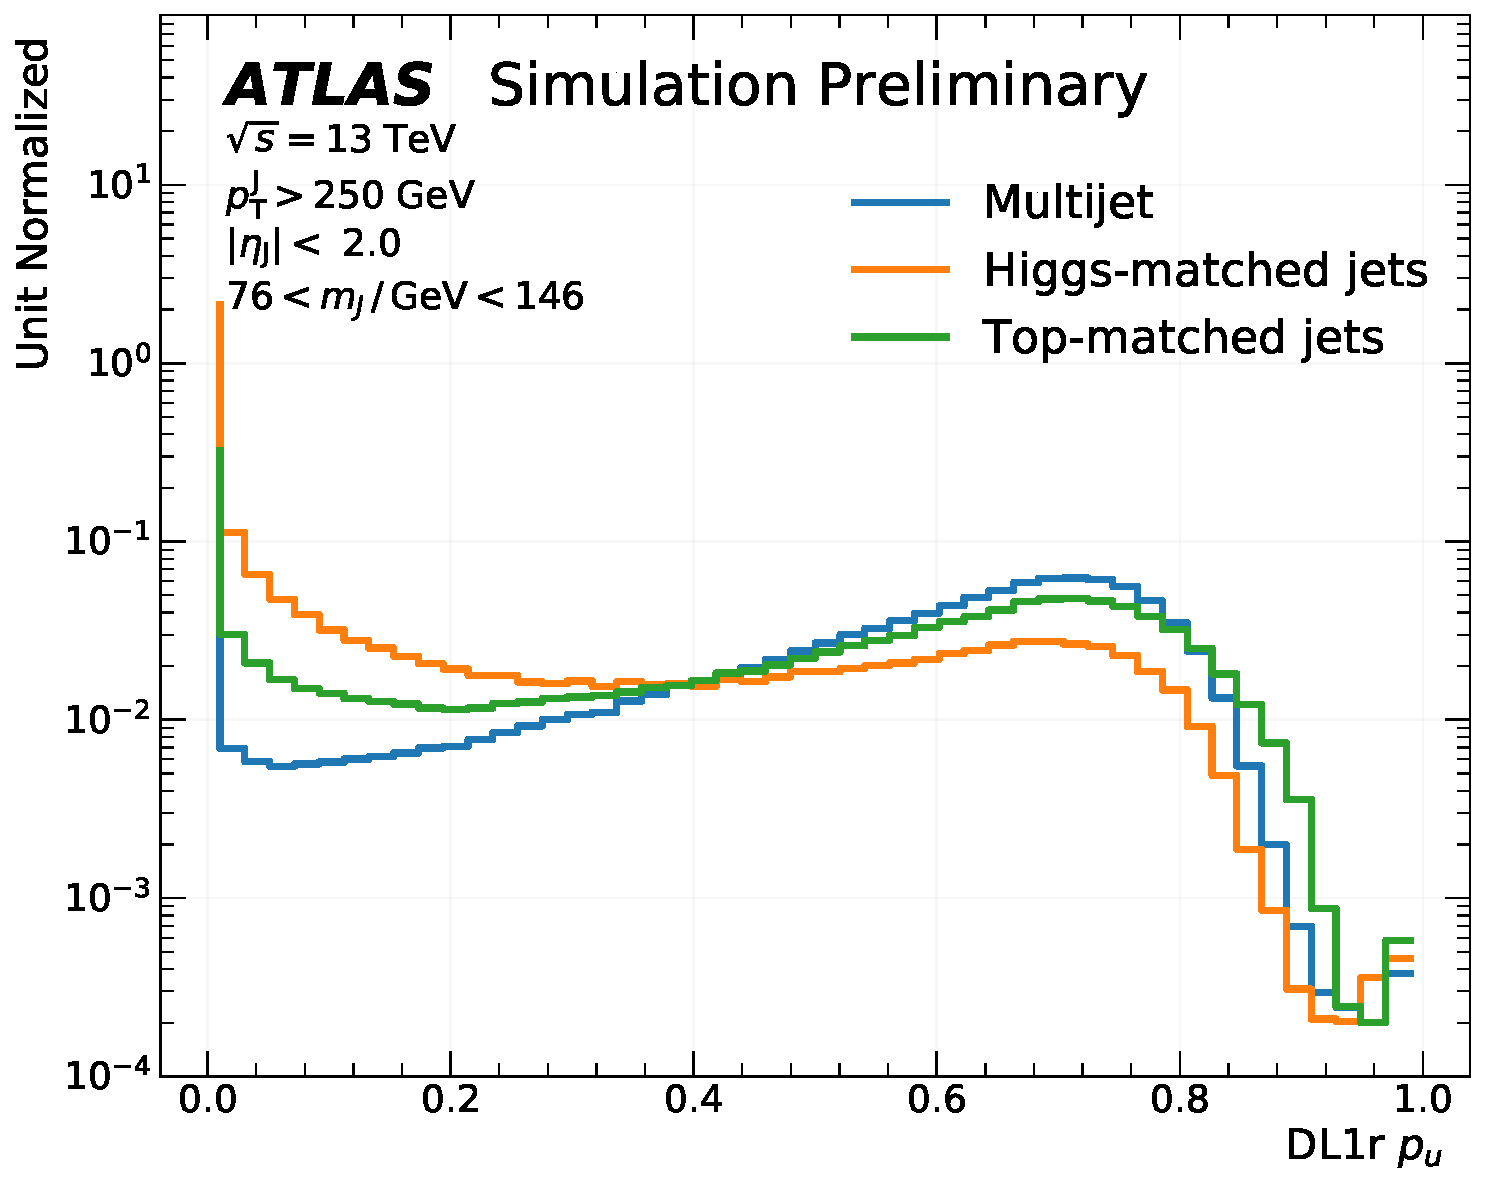
\includegraphics[width=0.33\textwidth]{figuresXbb/samples/inputs_aux/dl1r_pu_2_norm.pdf}
  \caption{在信号样本、multijet样本和t夸克样本中,领头LR-jet中的次领头也就是横动量第二高的VR-jet的DL1r算法输出值$p_b$、$p_c$和$p_u$的分布。
其中左图代表$p_b$的分布,中间的图代表$p_c$的分布,右图代表$p_u$的分布,橙色线代表信号样本,蓝色线代表multijet样本,绿色线代表t夸克样本。
所有分布都已经归一化。}
\label{fig:DL1RLLD}
\end{figure}

\begin{figure}[h]
    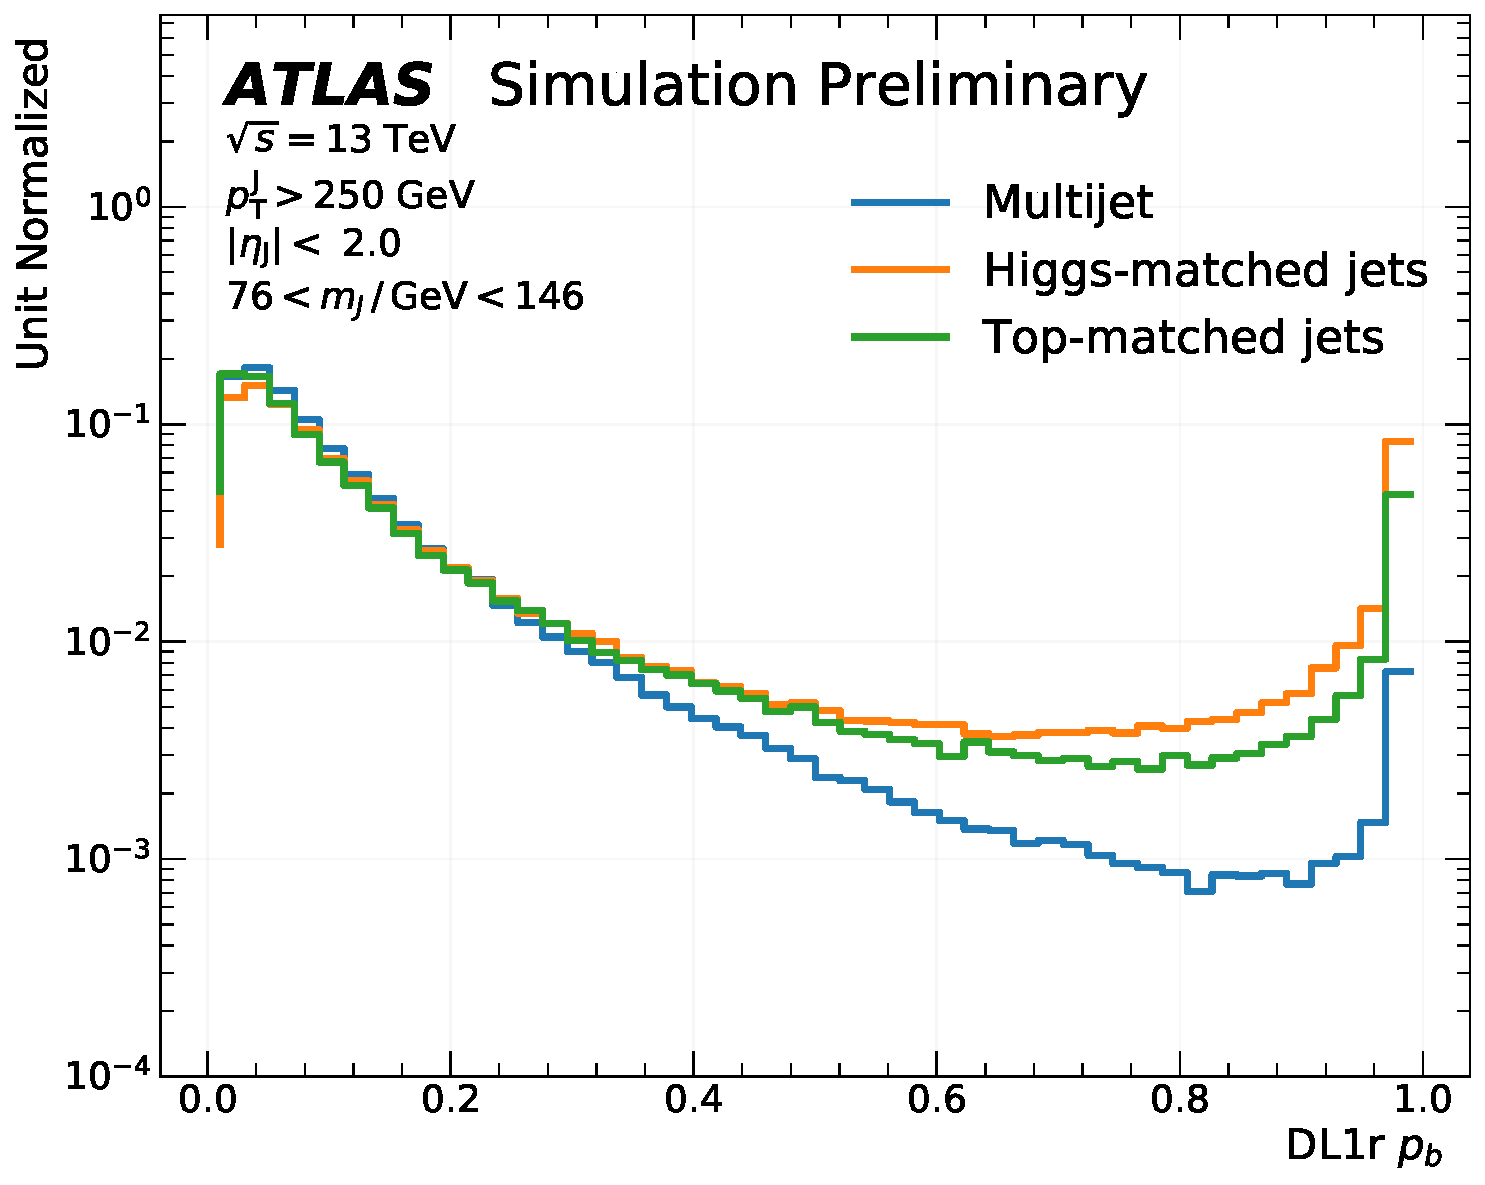
\includegraphics[width=0.33\textwidth]{figuresXbb/samples/inputs_aux/dl1r_pb_3_norm.pdf}
    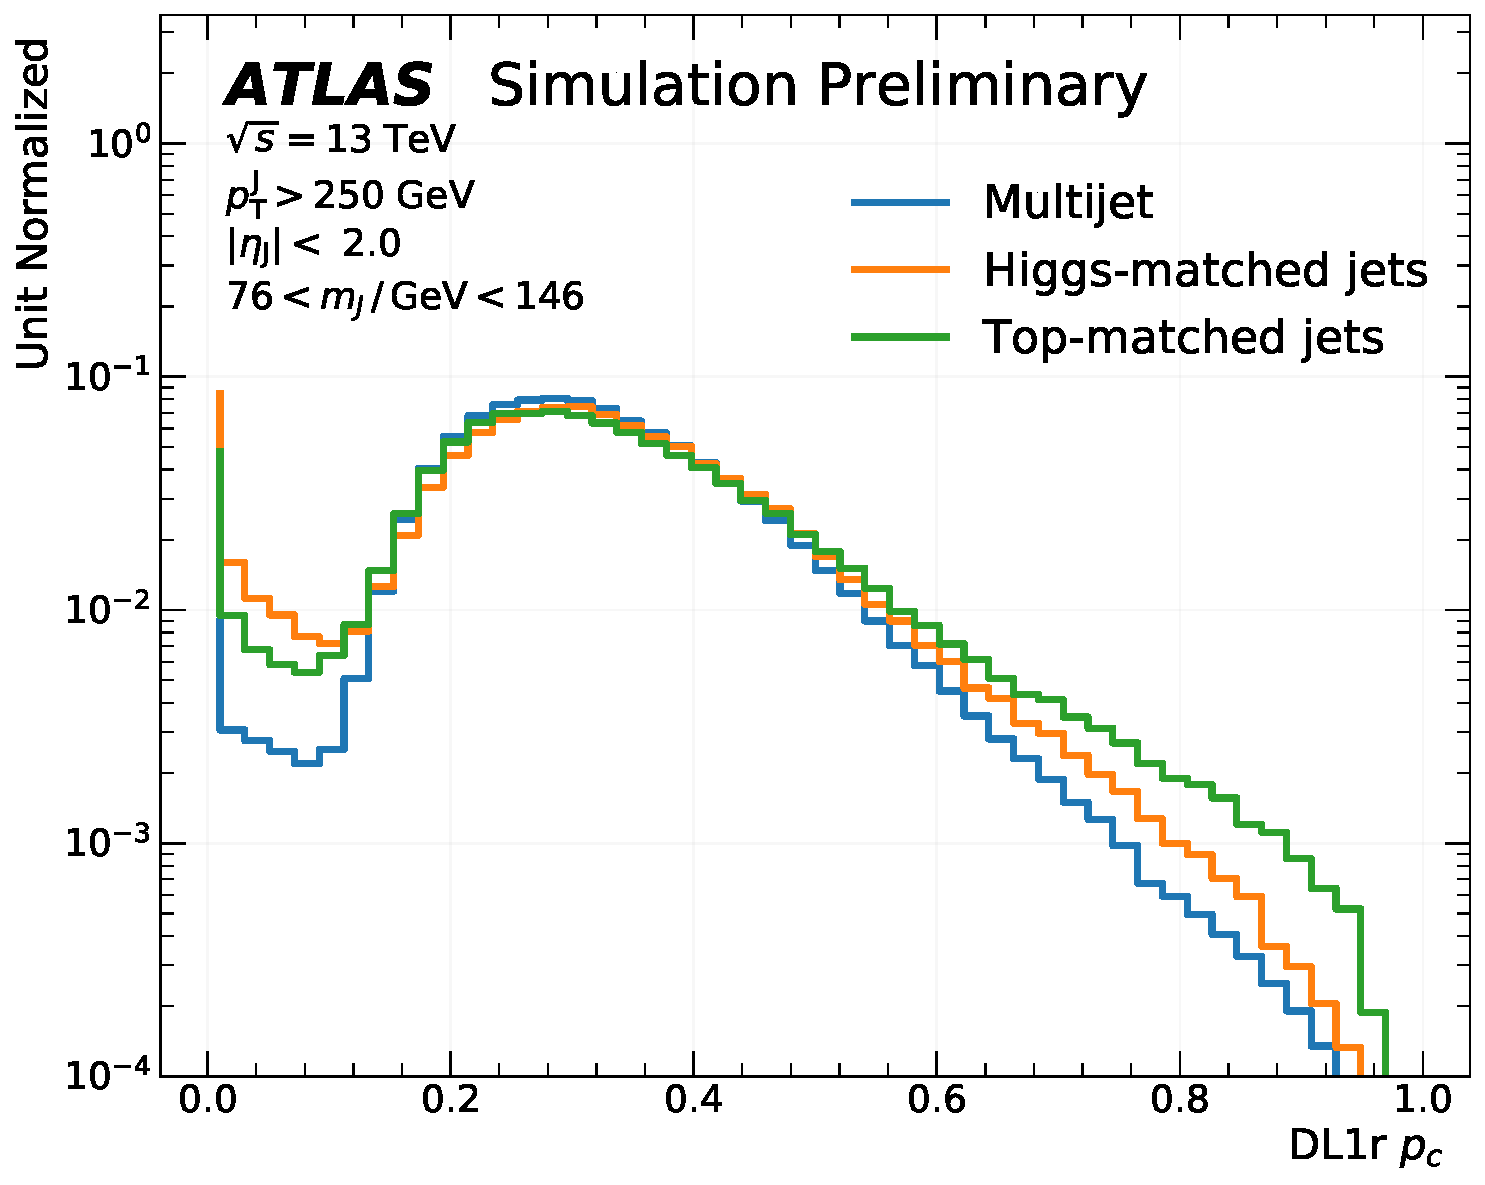
\includegraphics[width=0.33\textwidth]{figuresXbb/samples/inputs_aux/dl1r_pc_3_norm.pdf}
    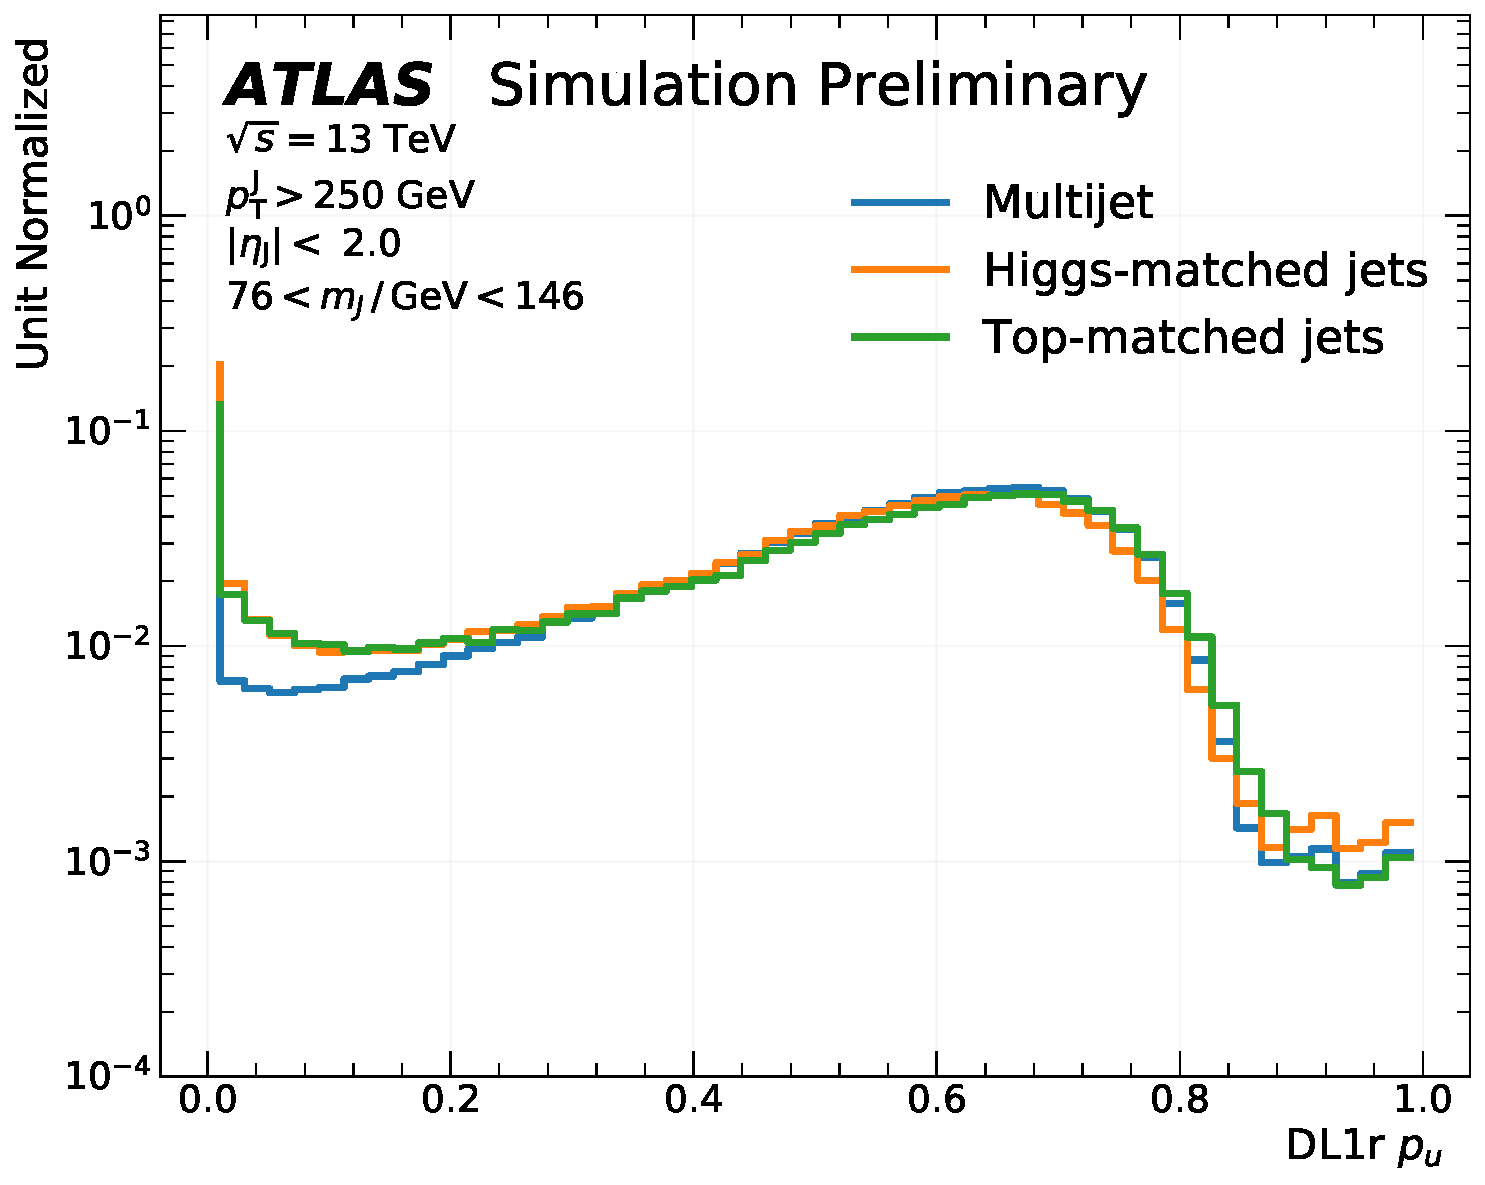
\includegraphics[width=0.33\textwidth]{figuresXbb/samples/inputs_aux/dl1r_pu_3_norm.pdf}
  \caption{在信号样本、multijet样本和t夸克样本中,领头LR-jet中的次次领头也就是横动量第三高的VR-jet的DL1r算法输出值$p_b$、$p_c$和$p_u$的分布。
其中左图代表$p_b$的分布,中间的图代表$p_c$的分布,右图代表$p_u$的分布,橙色线代表信号样本,蓝色线代表multijet样本,绿色线代表t夸克样本。
所有分布都已经归一化。}
\label{fig:DL1RLLLD}
\end{figure}


\begin{figure}[h]
    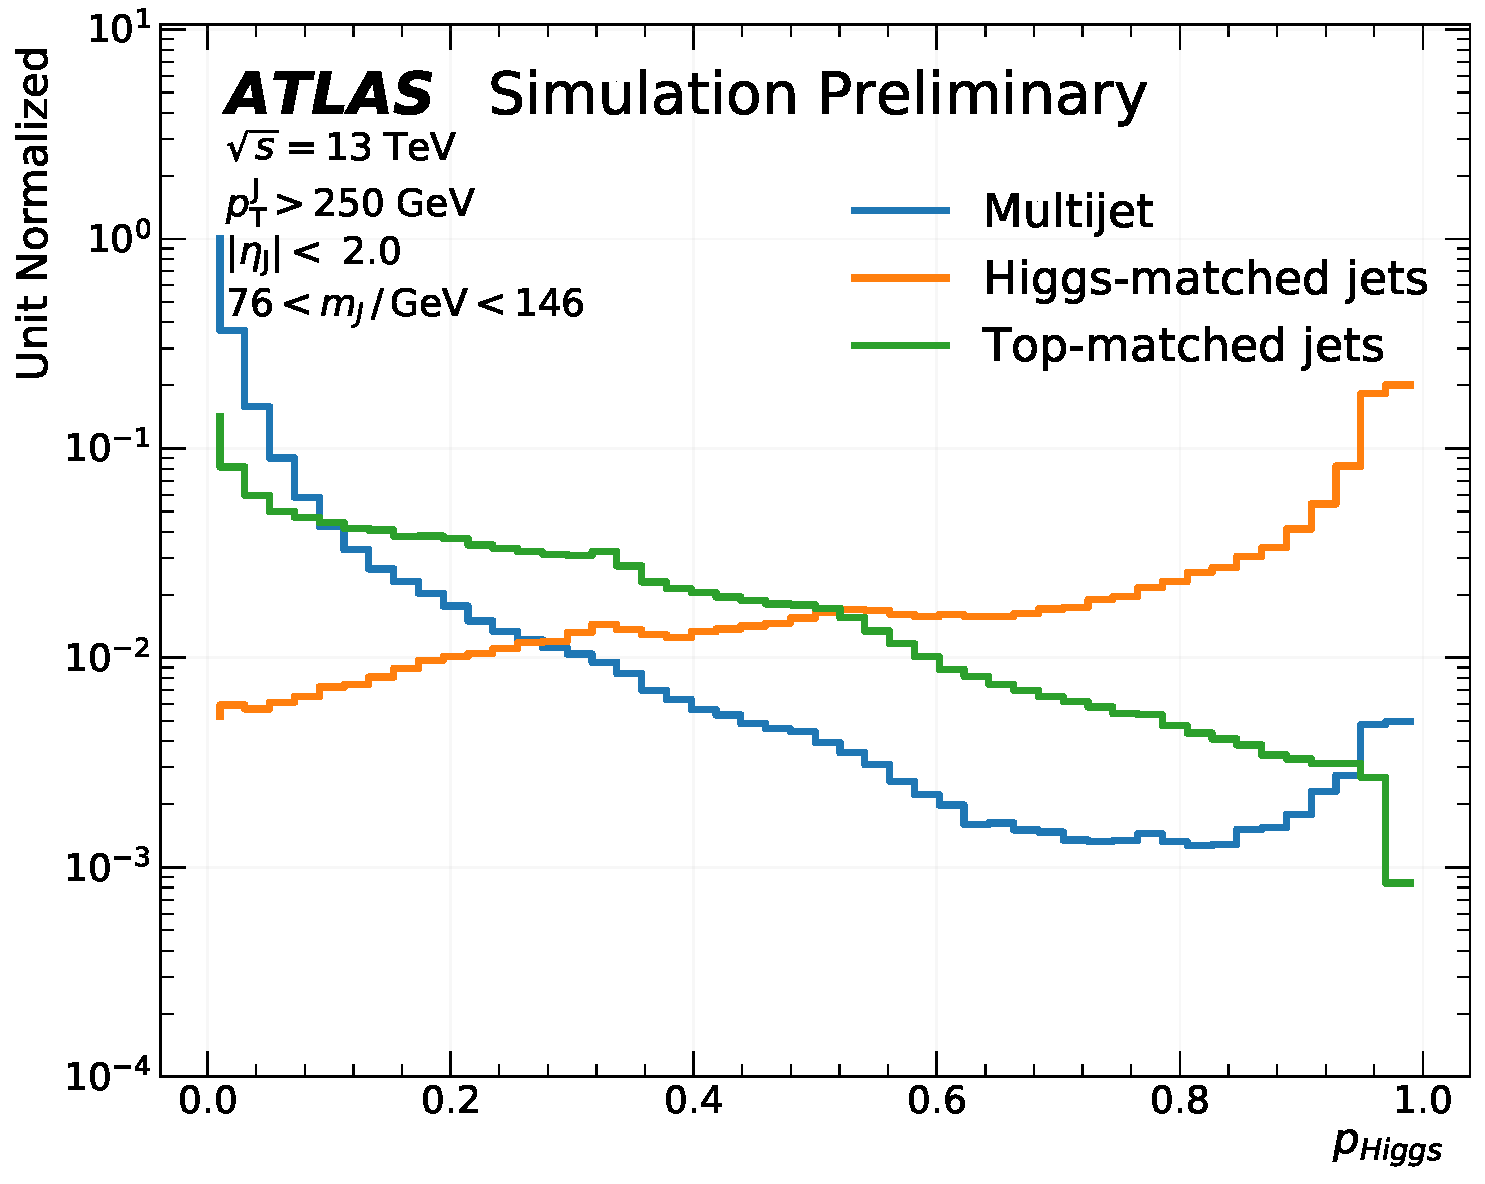
\includegraphics[width=0.33\textwidth]{figuresXbb/samples/probs_aux/Xbb_Higgs_norm.pdf}
    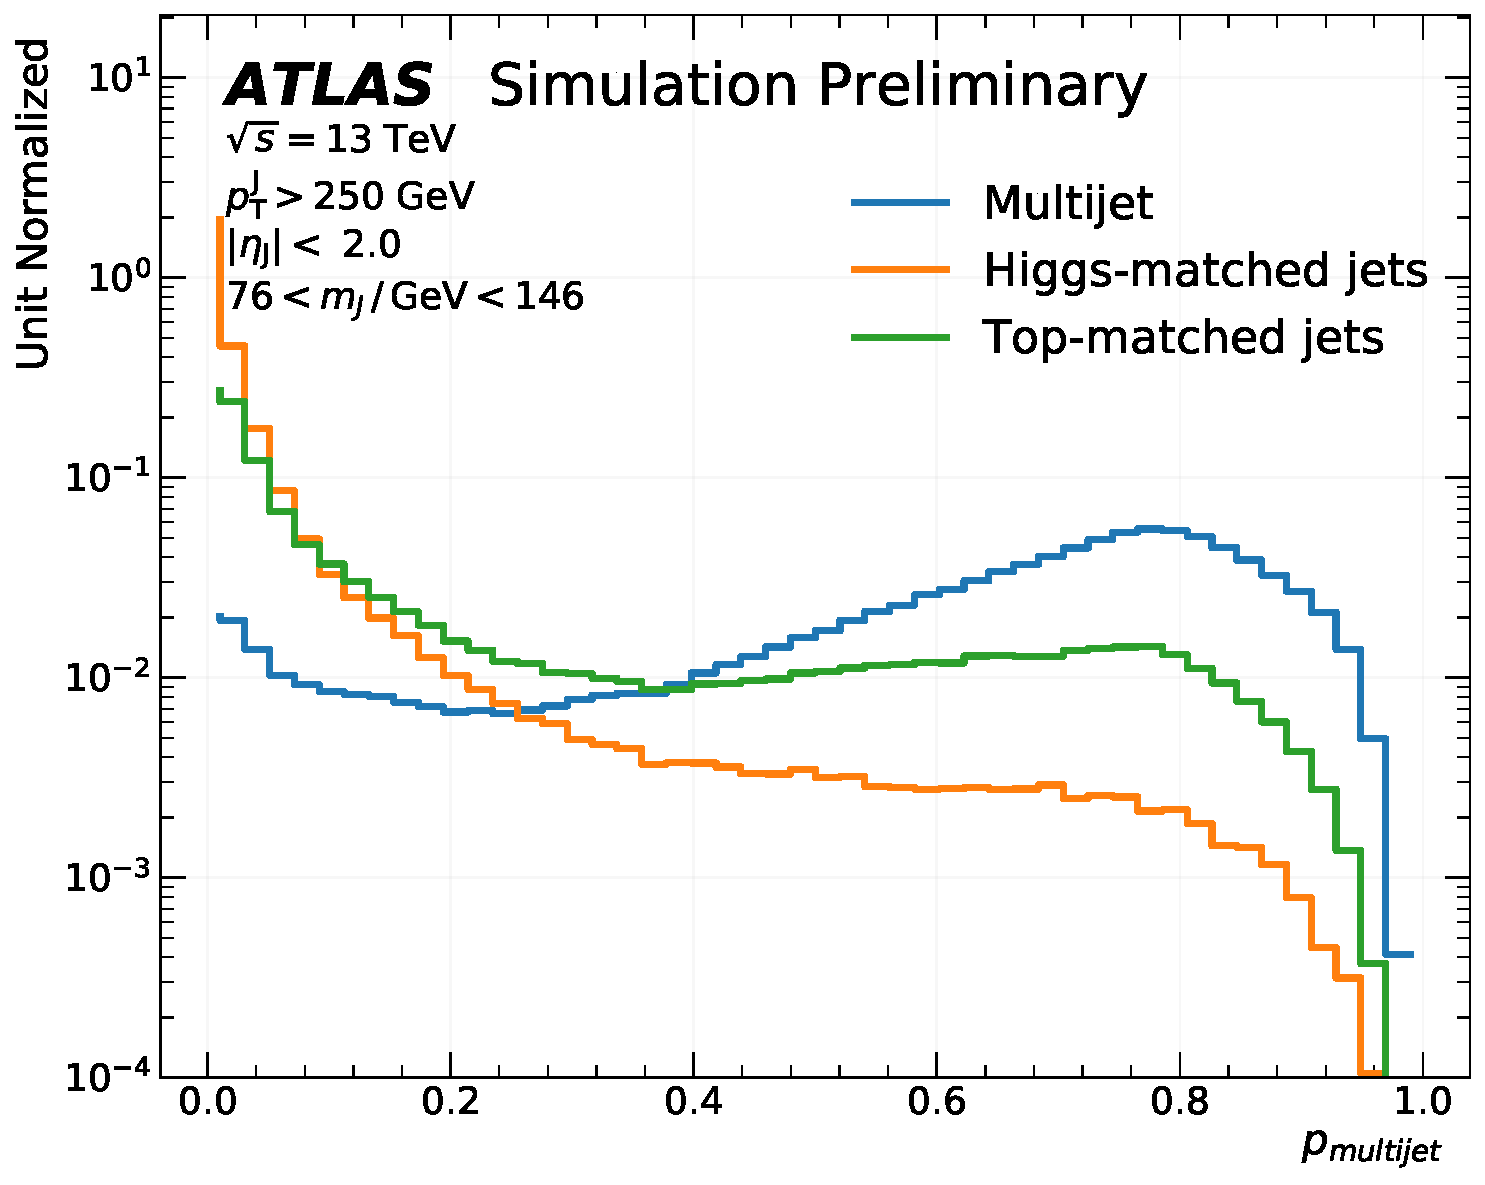
\includegraphics[width=0.33\textwidth]{figuresXbb/samples/probs_aux/Xbb_QCD_norm.pdf}
    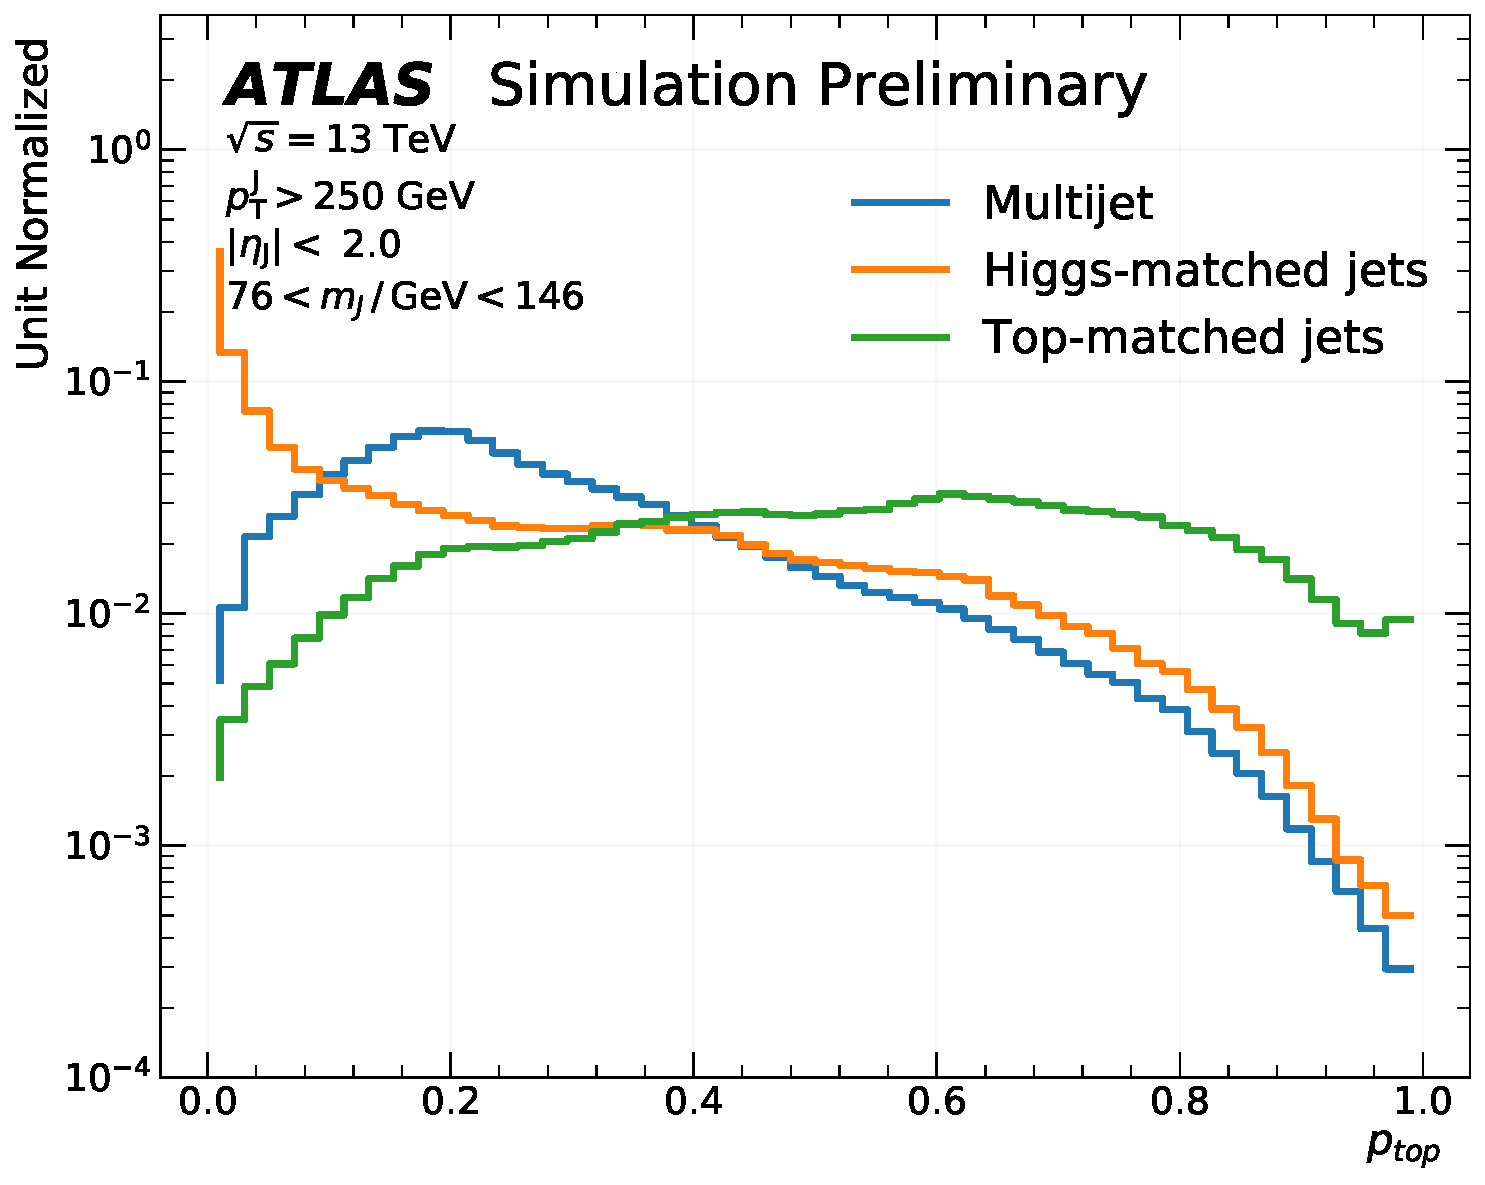
\includegraphics[width=0.33\textwidth]{figuresXbb/samples/probs_aux/Xbb_Top_norm.pdf}
  \caption{在信号样本、multijet样本和t夸克样本中,领头LR-jet中的新算法输出值$p_{\text{Higgs}}$、$p_{\text{multijet}}$和$p_{\text{top}}$的分布。
其中左图代表$p_{\text{Higgs}}$的分布,中间的图代表$p_{\text{multijet}}$的分布,右图代表$p_{\text{top}}$的分布,橙色线代表信号样本,蓝色线代表multijet样本,绿色线代表t夸克样本。
所有分布都已经归一化。}
  \label{fig:DXBBPP}
\end{figure}

